\section{Results} \label{sec:results}
\subsection{RQ1: Can we quantify interest of technical debt at the method-level?}
\smallsection{Motivation}
To alleviate the impact of technical debt, there are several previous studies on understanding SATD (e.g., the detection of technical debt~\cite{Potdar2014ICSME,Zazworka2013EASE} and the impact of SATD on software quality~\cite{Wehaibi2016SANER}).
However, there are few empirical studies that quantify interest of SATD.
Therefore, we would like to know how we can understand interest using our method explained in Section \ref{subsec:interest}

\smallsection{Approach}
%\para{We calculate the interest.}
To calculate interest of SATD, we follow the approach we explained in Section \ref{sec:setup}.
We show the number of SATD, the percentage of the technical debt that has positive interest, and the distribution of interest for technical debt of positive rate.

\smallsection{Results}
We find that there are high correlations between LOC and the other product metrics except Fan-In. 
From the highly correlated metrics, we choose LOC as metrics to calculate interest, similar to previous work that considers effort in the domain of defect prediction~\cite{Kamei2010ICSM,Kamei2013TSE}. We assume that developers spend more effort to check larger methods before modifying the methods. Eventually, we show our results using two product metrics (i.e., LOC and Fan-In).

Table \ref{tab:statistic} shows the number of SATD and the percentage of the technical debt that has positive interest in all technical debt. The table shows that 32.6\%-44.2\% of technical debt has a positve rate in terms of LOC and 30.9\%-42.2\% of technical debt has it in terms of Fan-In. 
There is not large difference of the positive rates between LOC and Fan-In. 
% The positive rate of LOC in ANT is 38.0% 

Figure \ref{fig:dist} and Table \ref{tab:statistic} show that the distribution of interest for the technical debt of positive rate. The distribution in LOC plots are left-skewed (around 0 to 10). We can also find that some of positive interest are over 100, which means the value of metric relatively increases by 100\%.
This findings suggest that we have the technical debt that we preferentially allocate development research to solve.

\begin{table}[tb]
  \caption{The percentage of SATD that has positive interest}
  \label{tab:percentage}
  \centering

  \begin{tabular}{cl|r|rrr}
  \hline
      &  Project & Positive Rate & All & Positive & Negative \\
  \hline
        & Ant    & 38.0\% &  71 &  27  &  20 \\
   LOC  & JMeter & 44.2\% & 181 &  80  &  25 \\
        & JRuby  & 32.6\% & 236 &  77  &  59 \\
  \hline
        & Ant    & 30.9\% &  68 &  21  &  13 \\
Fan-In  & JMeter & 42.2\% & 161 &  68  &  13 \\
        & JRuby  & 30.3\% & 231 &  70  &  37 \\
  \hline
  \end{tabular}
\end{table}

\begin{table}[tb]
  \caption{Statistics}
  \label{tab:statistic}
  \centering

  \begin{tabular}{cl|rrrrr}
  \hline
      &  Project & Min. & 1st Qu. & Median & 3rd Qu. & Max. \\
  \hline
        & Ant    & 1.4 &   6.2 &  11.1  &   25.4 &   75.0 \\
   LOC  & JMeter & 1.6 &   6.9 &  18.0  &   50.0 & 6667.0 \\
        & JRuby  & 1.3 &   7.5 &  20.7  &   40.0 &  362.5 \\
  \hline
        & Ant    & 5.3 &  20.0 &  33.3  &  100.0 & 2700.0 \\
Fan-In  & JMeter & 5.6 &  12.4 &  25.0  &   50.0 &  900.0 \\
        & JRuby  & 7.1 &  17.5 &  33.3  &  100.0 &  450.0 \\
  \hline
  \end{tabular}
\end{table}

%-----------------------------------------------------------------------
\begin{figure*}[!t]
  \begin{center}
  \scalebox{0.95}{
  \begin{tabular}{ccc}
    \subfigure[Ant (LOC)]{ 
      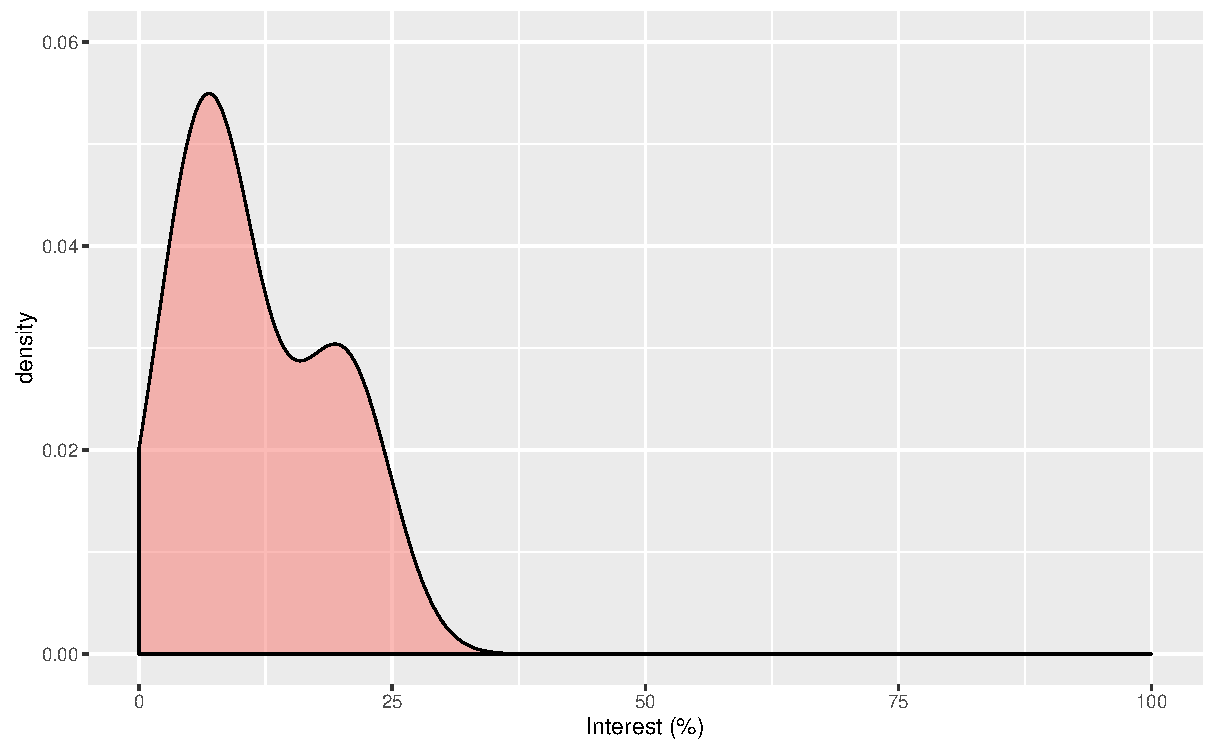
\includegraphics[width=.33\textwidth]{figures/rq1-ant}
    }
    \subfigure[JMeter (LOC)]{ 
      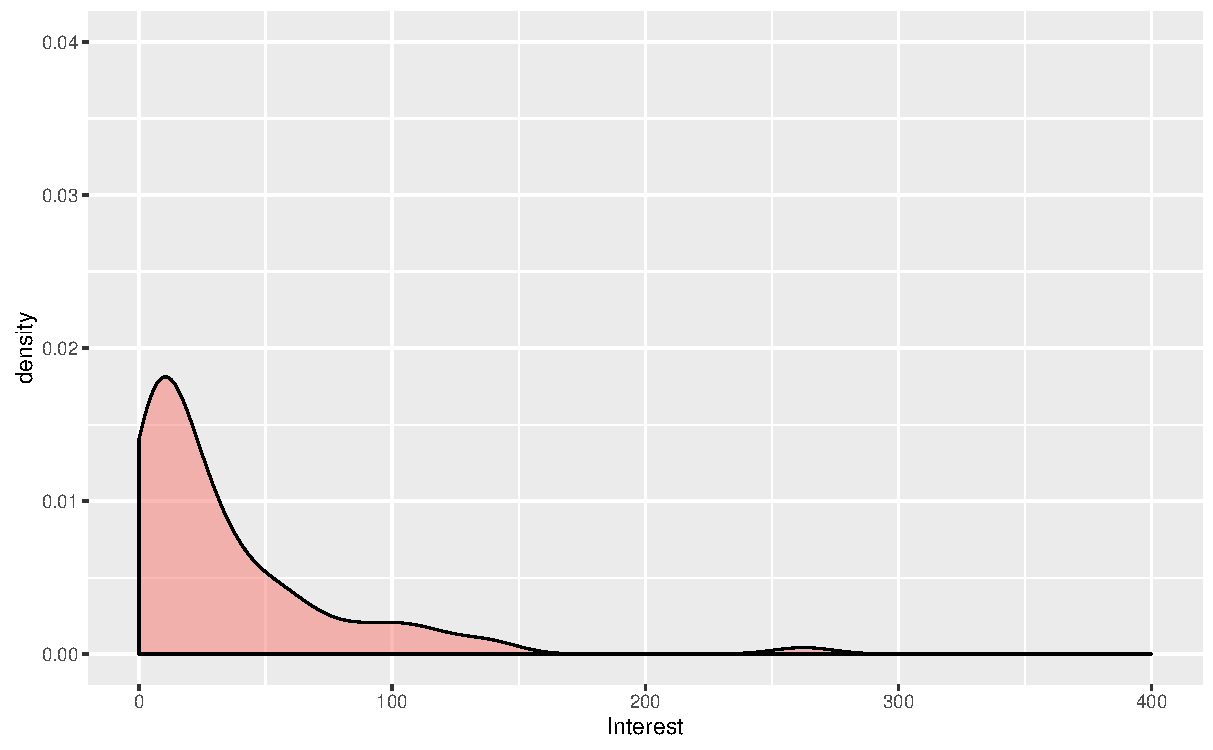
\includegraphics[width=.33\textwidth]{figures/rq1-jmeter}
    }
    \subfigure[JRuby (LOC)]{
      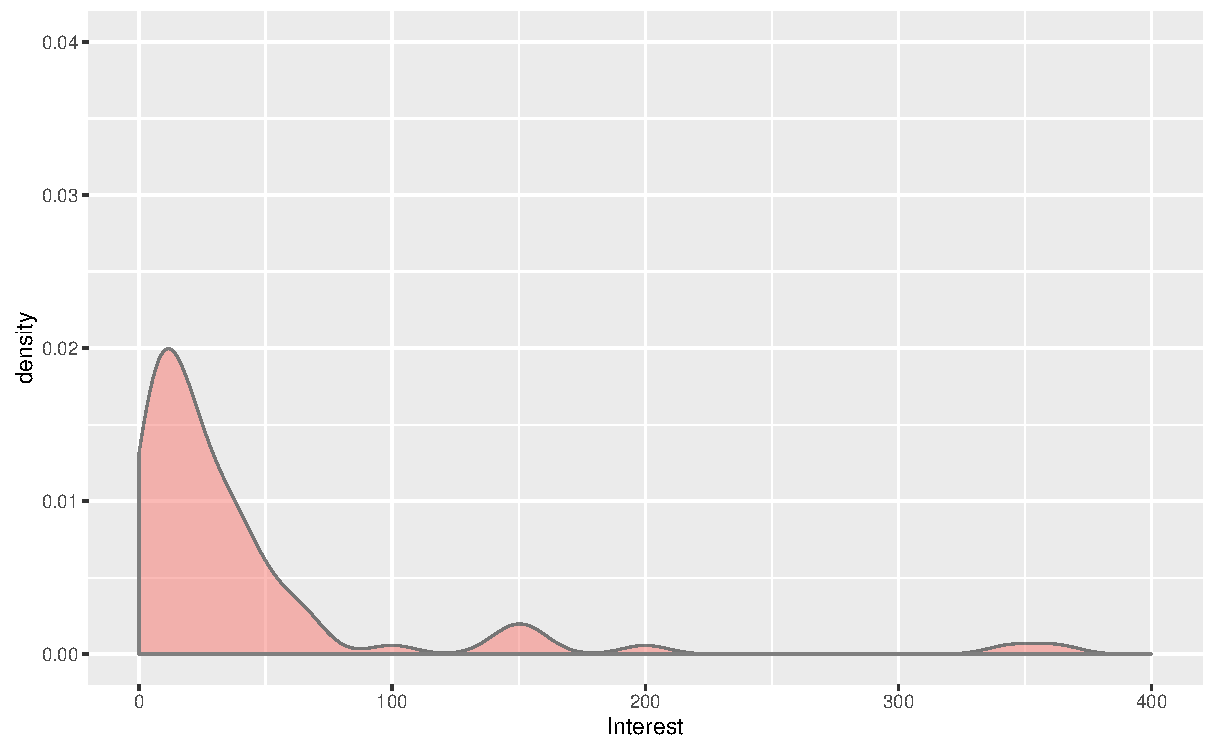
\includegraphics[width=.33\textwidth]{figures/rq1-jruby}
    }
  \end{tabular}
  }
  \scalebox{0.95}{
  \begin{tabular}{ccc}
    \subfigure[Ant (Fan-In)]{ 
      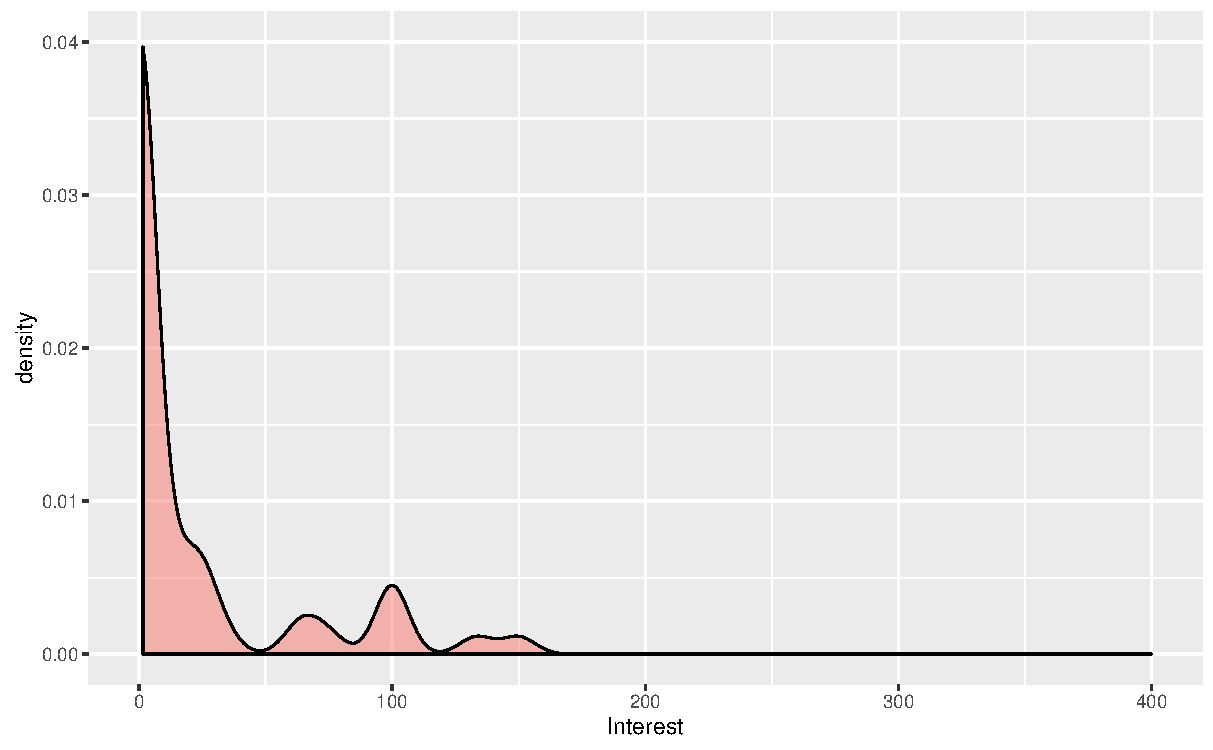
\includegraphics[width=.33\textwidth]{figures/rq1-ant-fanin}
    }
    \subfigure[JMeter (Fan-In)]{ 
      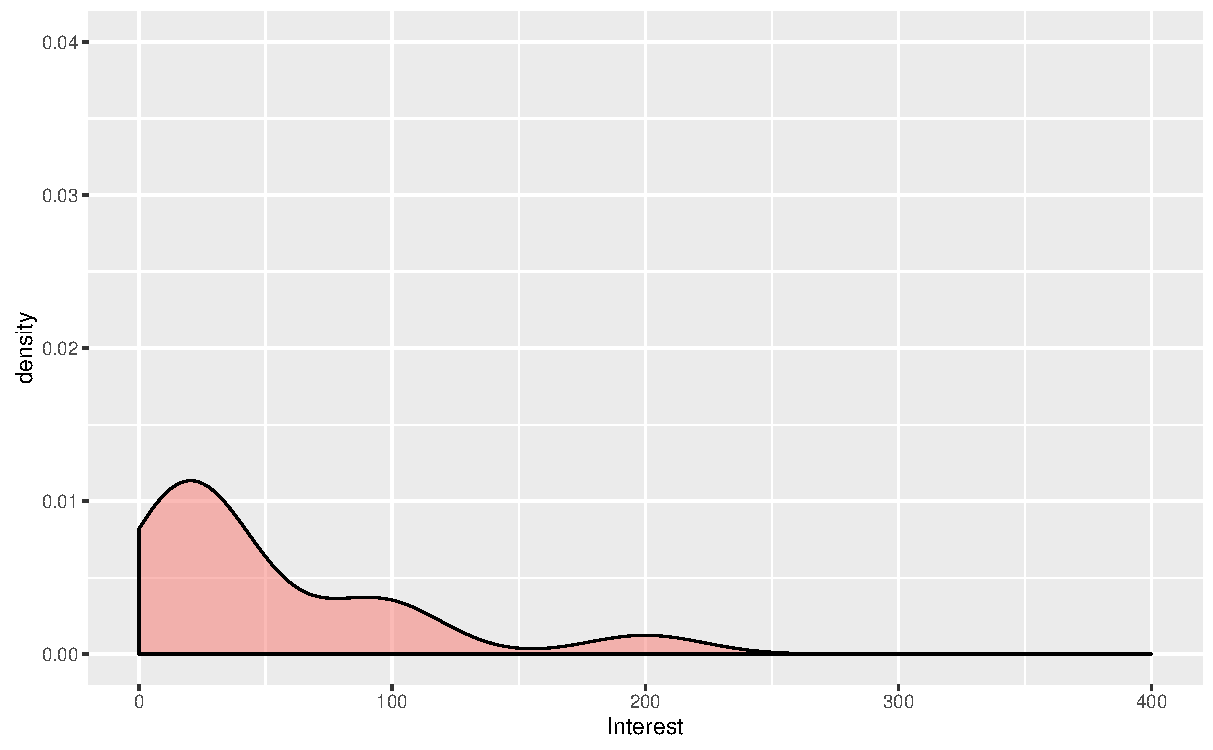
\includegraphics[width=.33\textwidth]{figures/rq1-jmeter-fanin}
    }
    \subfigure[JRuby (Fan-In)]{
      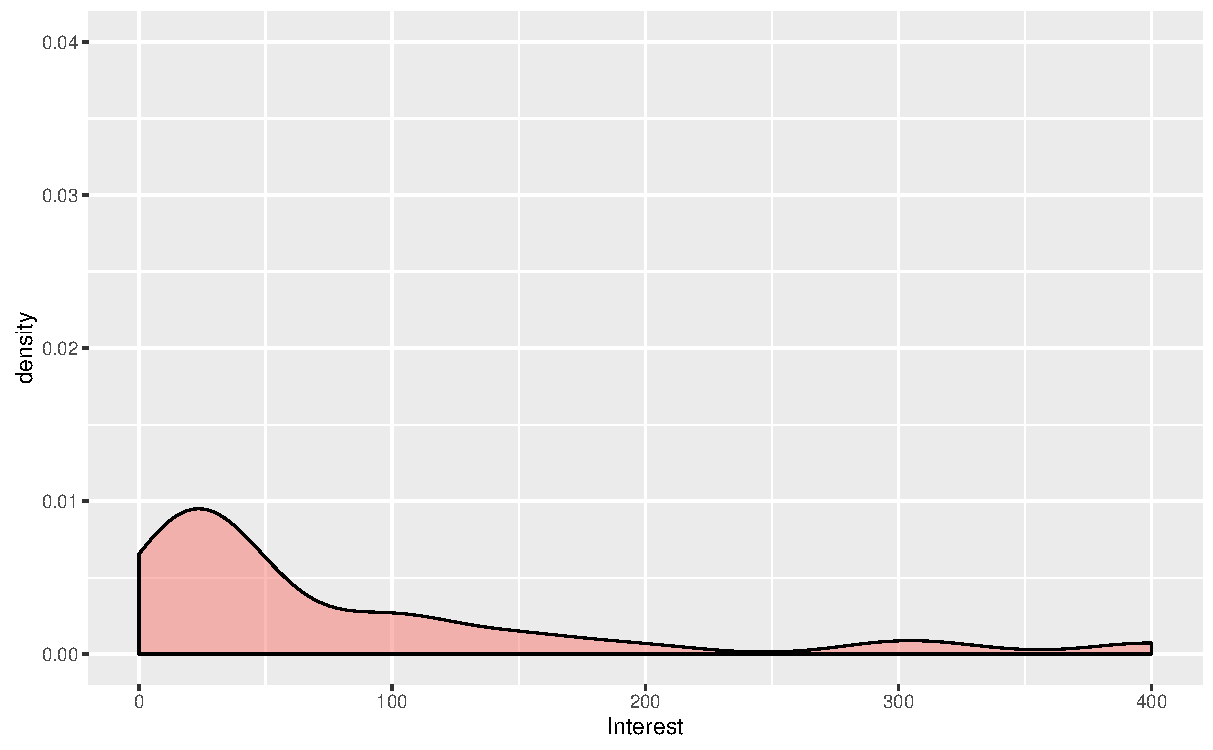
\includegraphics[width=.33\textwidth]{figures/rq1-jruby-fanin}
    }
  \end{tabular}
  }
  \caption{(RQ1) The results of distribution of interest.}
  \label{fig:dist}
  \end{center}
\end{figure*}
%-----------------------------------------------------------------------


\conclusionbox{
32.6\%-44.2\% of technical debt has a positive rate in terms of LOC and 30.9\%-42.2\% of technical debt has it in terms of Fan-In.}

\subsection{RQ2: Does the interest differ based on the type of technical debt?}
\smallsection{Motivation}
There are several type of technical debt such as defect technical debt and design technical debt.
The previous study~\cite{Maldonado2015MTD} shows that the percentage of technical debt varies depending on the type of technical debt and the studied systems. For example, the projects that have limited time to develop features are likely to leave comments of features that need to be implemented in the future. 
To better understand the interest, we would like to analyze the interest per type of technical debt.

\smallsection{Approach}
We manually classify technical debt into five categories (i.e., Design, Defect, Requirement, Test, and Documentation)~\cite{Maldonado2015MTD}. {\bf Design debt} indicates that there is a problem with the design of the code, and {\bf Defect debt} states that a part of the code does not have the expected behavior. {\bf Documentation debt} expresses that there is no proper documentation supporting that part of the program. {\bf Requirement debt} shows that incompleteness of the method, class or program. {\bf Test debt} indicates the need for implementation or improvement of the current tests.

Similar to RQ1, we show the number of SATD, the percentage of the technical debt that has positive interest, and the distribution of interest for technical debt of positive rate.

\smallsection{Results}
Among three projects, JRuby only includes more than one category that has more than 10\% of technical debt methods. For example, in the JMeter Project, 82\% of technical debt are categorized as design debt. Therefore, we decided to use JRuby in RQ2, because the types of technical debt in the others are skewed in one category.

Table \ref{tab:percentage_type} and \ref{tab:statistic_type}

Figure \ref{fig:type} shows the number and the percentage of technical debt. 


\begin{table}[tb]
  \caption{(RQ2) The percentage of SATD that has positive interest per type}
  \label{tab:percentage_type}
  \centering

  \begin{tabular}{cl|r|rrr}
  \hline
      &  Type & Positive Rate & All & Positive & Negative \\
  \hline
        & Defect & 30.5\% &  87 &  25  &  16 \\
   LOC  & Design & 38.9\% & 108 &  42  &  30 \\
        & Requirement & 24.3\% & 37 & 9 & 11 \\
  \hline
        & Defect    & 19.8\% & 86 & 17  &   5 \\
Fan-In  & Design & 38.0\% & 106 &  41  &   18 \\
        & Requirement  & 31.4\% & 35 & 11 & 12 \\
  \hline
  \end{tabular}
\end{table}

\begin{table}[tb]
  \caption{(RQ2) Statistics}
  \label{tab:statistic_type}
  \centering

  \begin{tabular}{cl|rrrrr}
  \hline
      &  Type & Min. & 1st Qu. & Median & 3rd Qu. & Max. \\
  \hline
        & Defect    & 6.3 &  20.0 &  36.4  &   56.3 &  200.0 \\
   LOC  & Design & 1.3 &   5.6 &  15.2  &   30.8 & 362.5 \\
        & Requirement  & 1.5 &   6.8 &  23.7  &   45.5 &  64.4 \\
  \hline
        & Defect    & 11.1 &  25.0 &  40.0  & 111.9 & 400.0 \\
Fan-In  & Design & 7.1 &  25.4 &  36.4  &  100.0 &  400.0 \\
        & Requirement  & 7.1 &  8.0 &  20.0  &  91.7 &  450.0 \\
  \hline
  \end{tabular}
\end{table}

\conclusionbox{Result of RQ2}

\subsection{RQ3: manual analysis}
\smallsection{Motivation}

\smallsection{Approach}

\smallsection{Results}

\conclusionbox{Result of RQ3}

%-----------------------------------------------------------------------
\begin{figure*}[!t]
  \begin{center}
  \scalebox{0.95}{
  \begin{tabular}{ccc}
    \subfigure[Defect (LOC)]{ 
      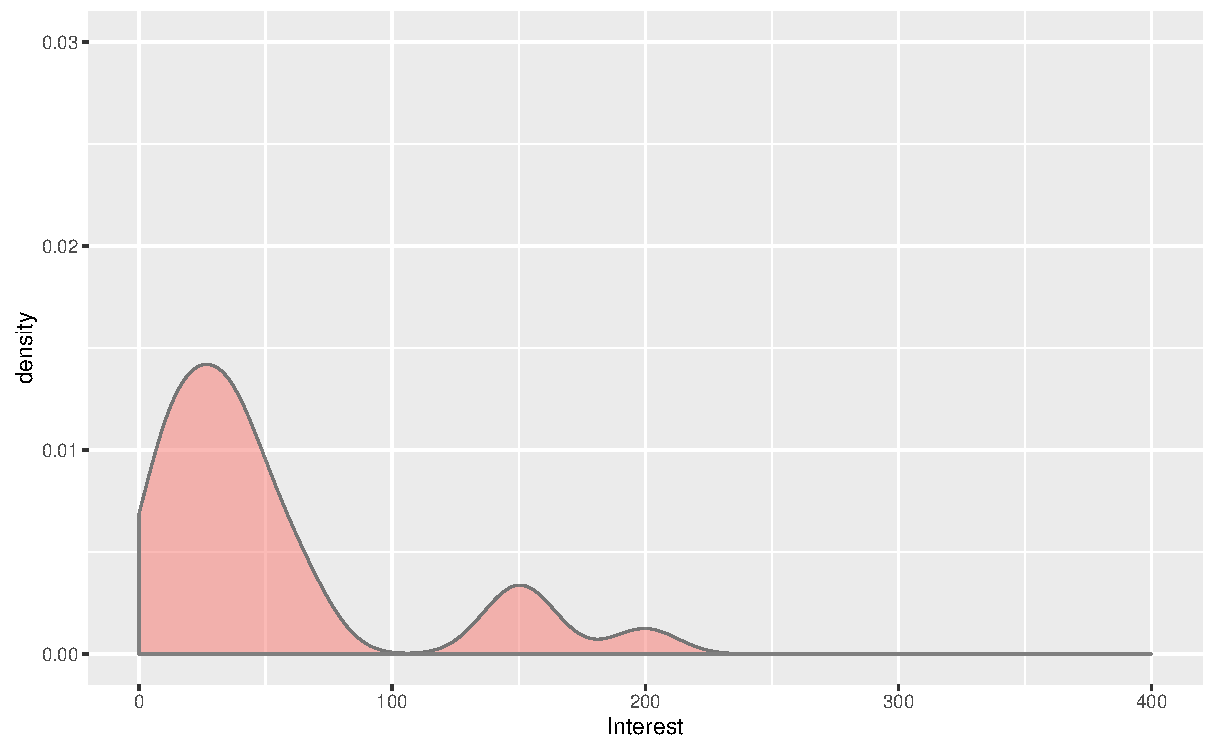
\includegraphics[width=.33\textwidth]{figures/rq2-defect}
    }
    \subfigure[Design (LOC)]{ 
      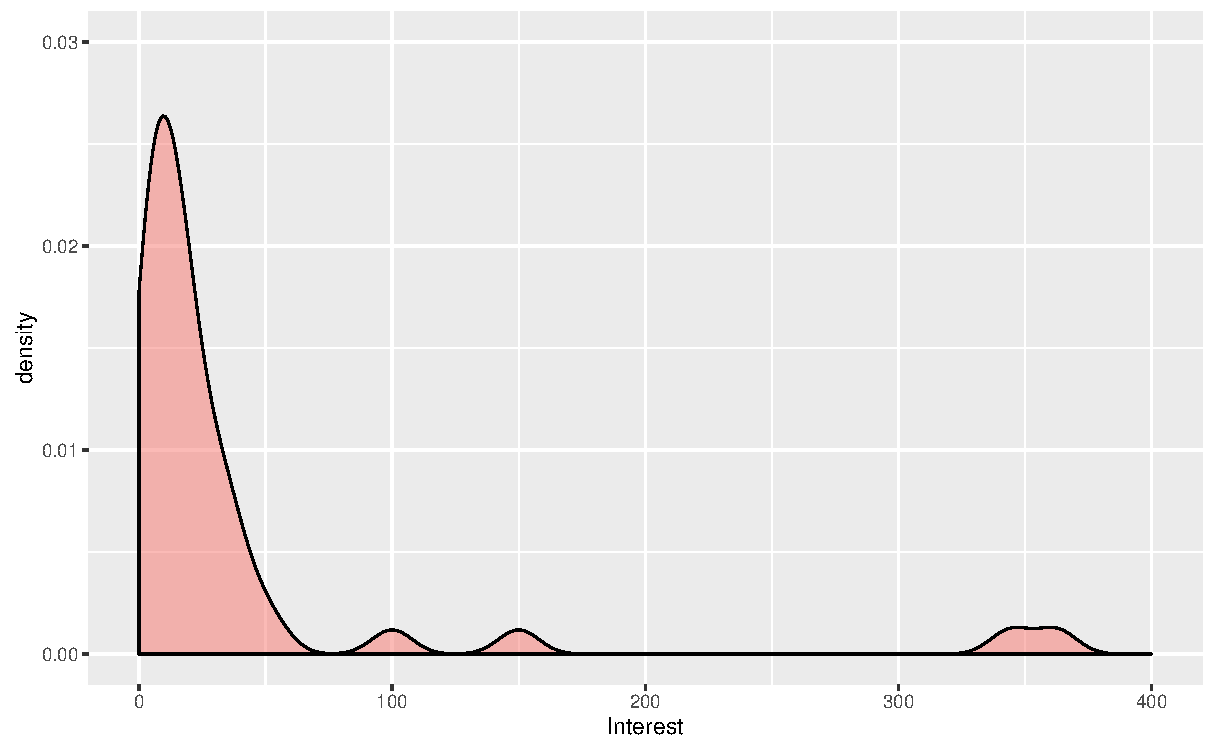
\includegraphics[width=.33\textwidth]{figures/rq2-design}
    }
    \subfigure[Requirement (LOC)]{
      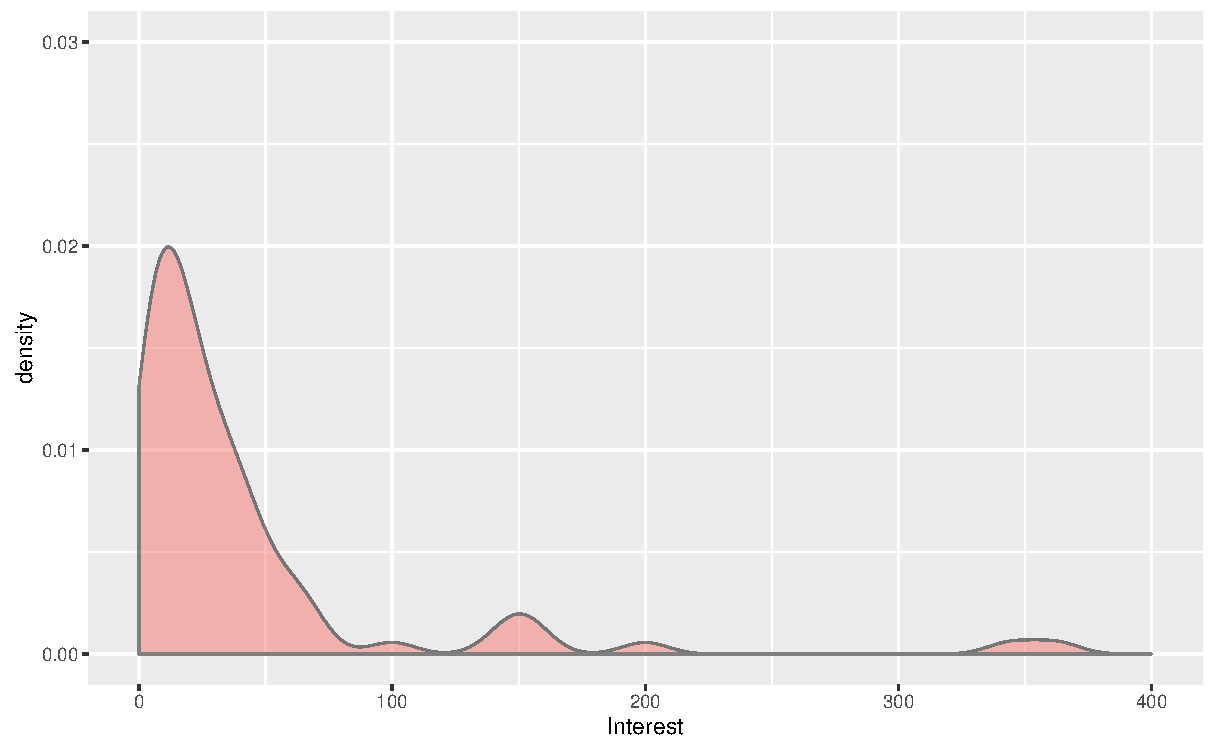
\includegraphics[width=.33\textwidth]{figures/rq2-requirement}
    }
  \end{tabular}
  }
  \scalebox{0.95}{
  \begin{tabular}{ccc}
    \subfigure[Defect (Fan-In)]{ 
      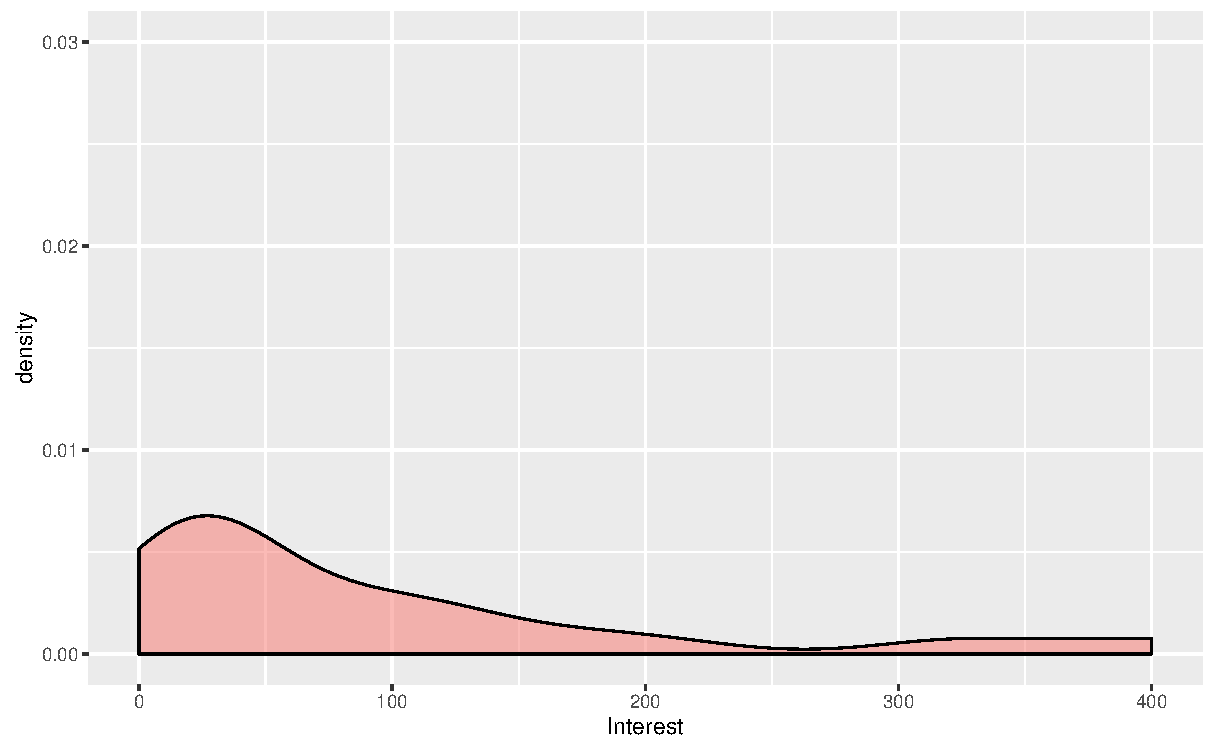
\includegraphics[width=.33\textwidth]{figures/rq2-defect-countinput}
    }
    \subfigure[Design (Fan-In)]{ 
      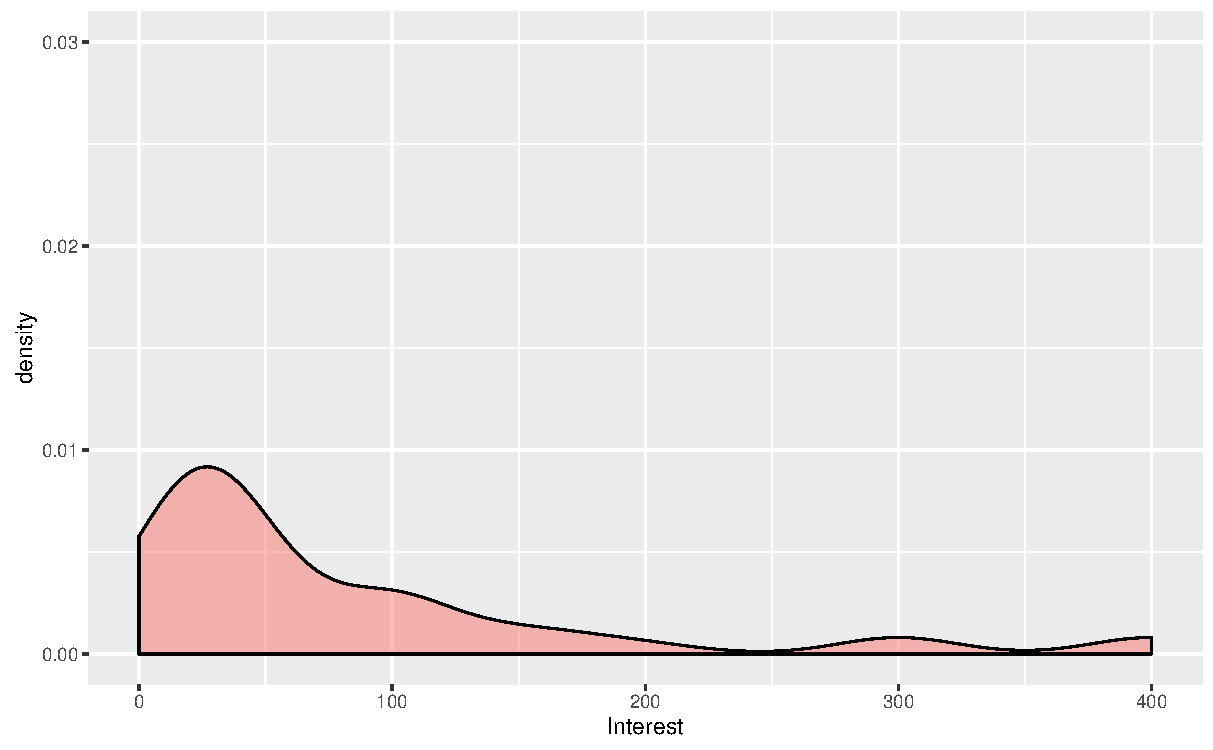
\includegraphics[width=.33\textwidth]{figures/rq2-design-countinput}
    }
    \subfigure[Requirement (Fan-In)]{
      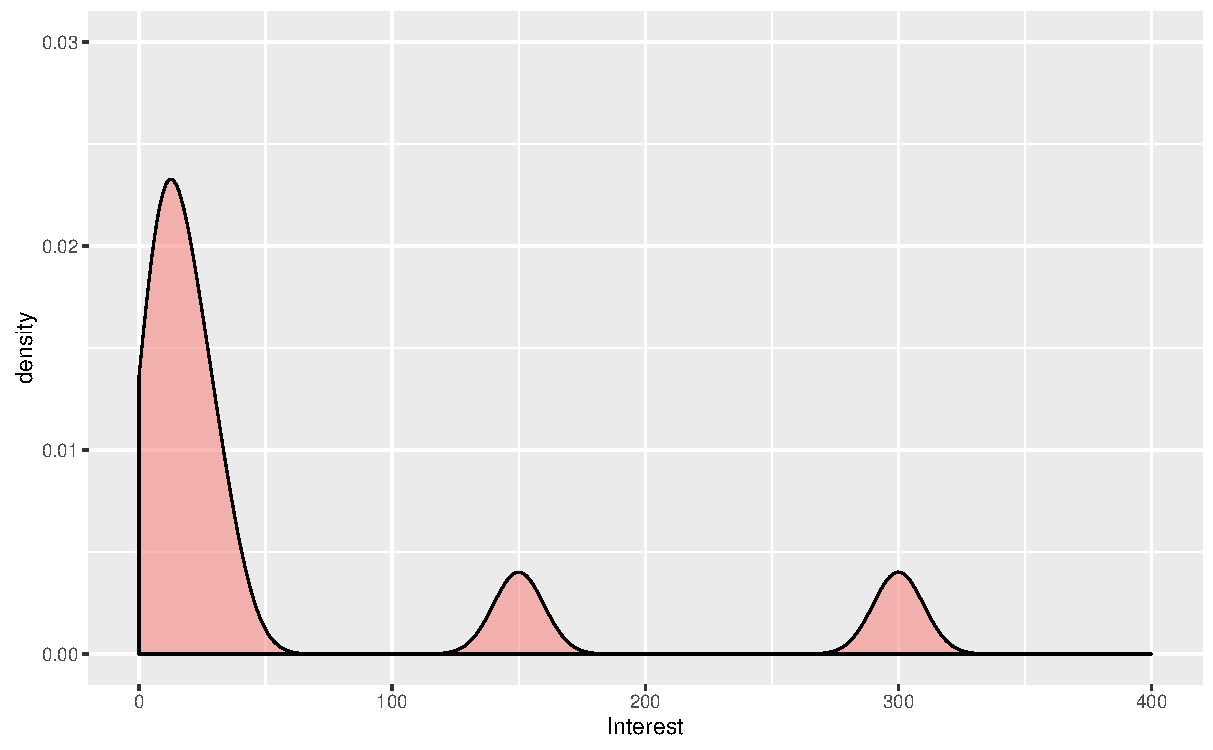
\includegraphics[width=.33\textwidth]{figures/rq2-requirement-countinput}
    }
  \end{tabular}
  }
  \caption{(RQ2) Distribution of interest per type in JRuby.}
  \label{fig:type}
  \end{center}
\end{figure*}
%-----------------------------------------------------------------------


\section{Discussion}
\para{Put additional analysis when considering time period.}

\para{Put additional analysis when considering other metrics (fan-in).}

%\para{Put additional analysis when comparing the non-technical deb methods.}
\smallsection{Motivation}
Generally speaking, software systems are always evolving over time for implementing new functionality and fixing defects~\cite{xxx}.
Therefore, even if the size of technical debt increases, it is not clear about how the nature of software evaluation affects the interest of technical debt.
We would like to compare the impact of software evolution on methods in two groups of SATD v.s. non-SATD.

\smallsection{Approach}
We compare the interest of methods between SATD and non-SATD.
We conduct the following steps:
\begin{itemize}
\item We obtain the list of files that include SATD. % from technical_debt_summary.csv
\item We extract methods that do not include SATD. % see .method-level.product.csv
\item We measure metrics for the methods in Step 2 at two versions that technical debt is introduced and removed.
\item We calculate interest using metrics in Step 3.
\end{itemize}
% What do we need to do some pre-condition for this analysis?

\smallsection{Result}
%-----------------------------------------------------------------------
\begin{figure*}[!t]
  \begin{center}
  \scalebox{0.95}{
  \begin{tabular}{ccc}
    \subfigure[Ant (LOC)]{ 
      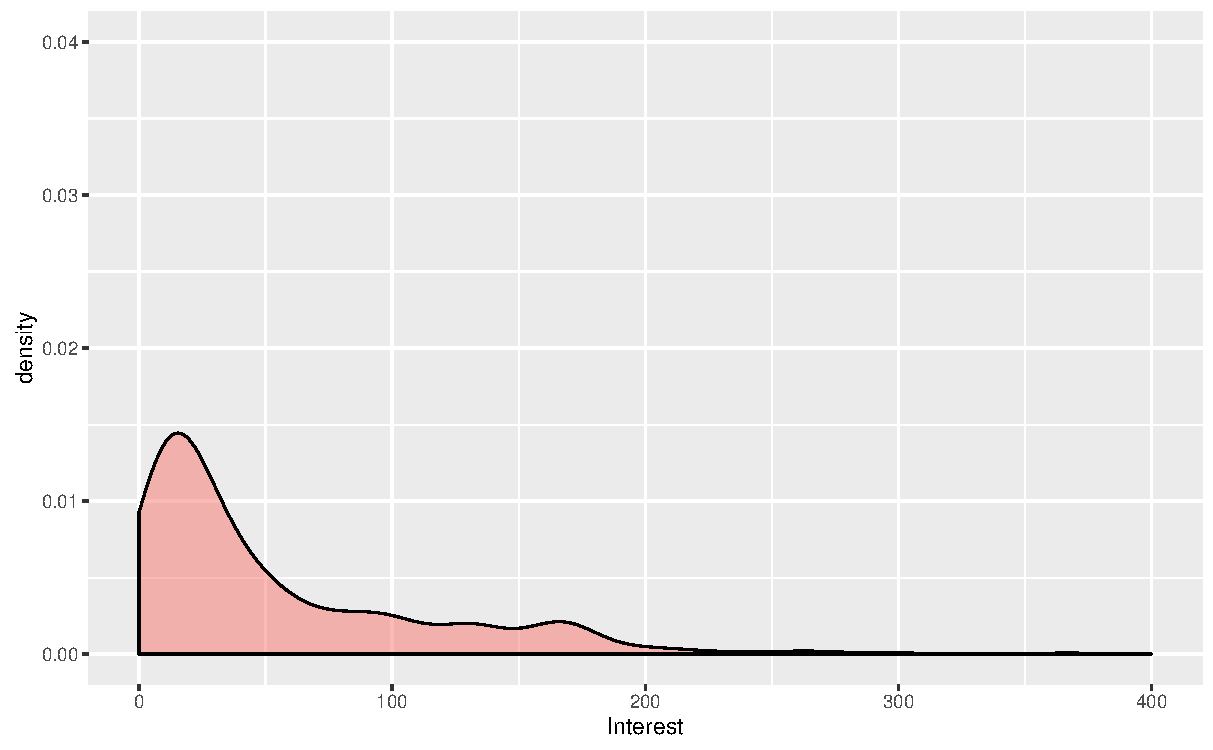
\includegraphics[width=.33\textwidth]{figures/rq1-ant-non-SATD}
    }
    \subfigure[JMeter (LOC)]{ 
      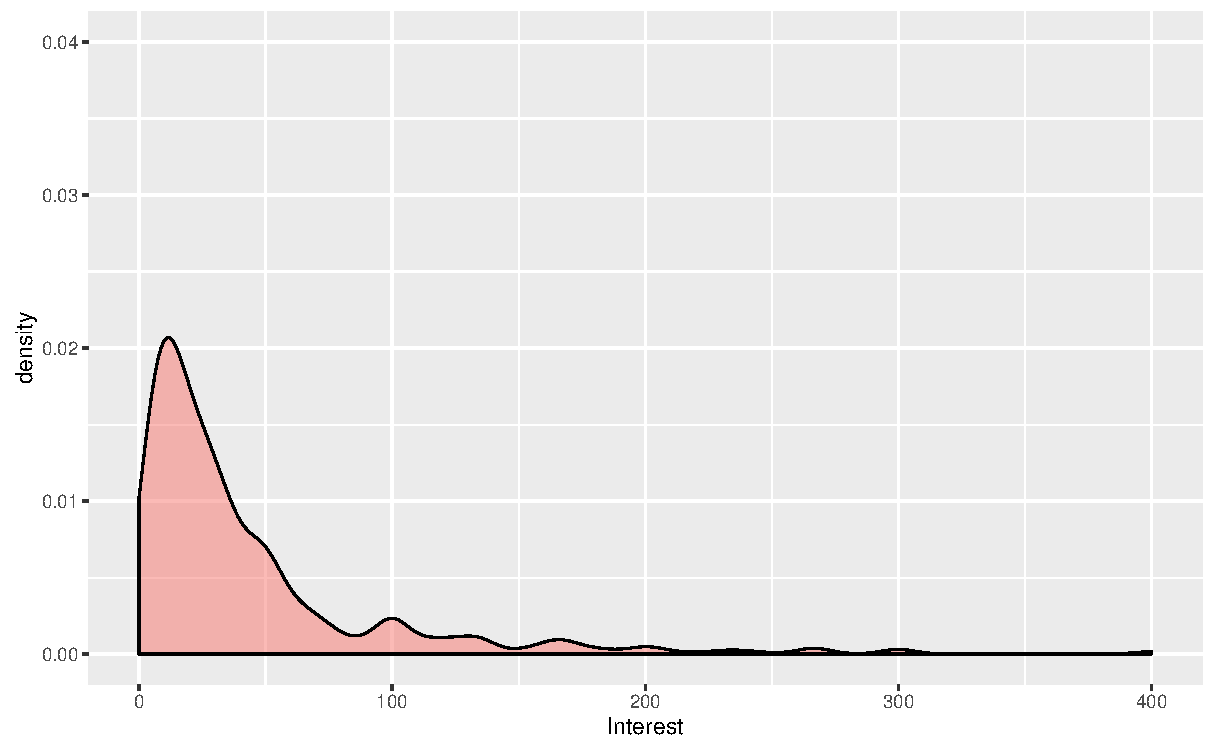
\includegraphics[width=.33\textwidth]{figures/rq1-jmeter-non-SATD}
    }
    \subfigure[JRuby (LOC)]{
      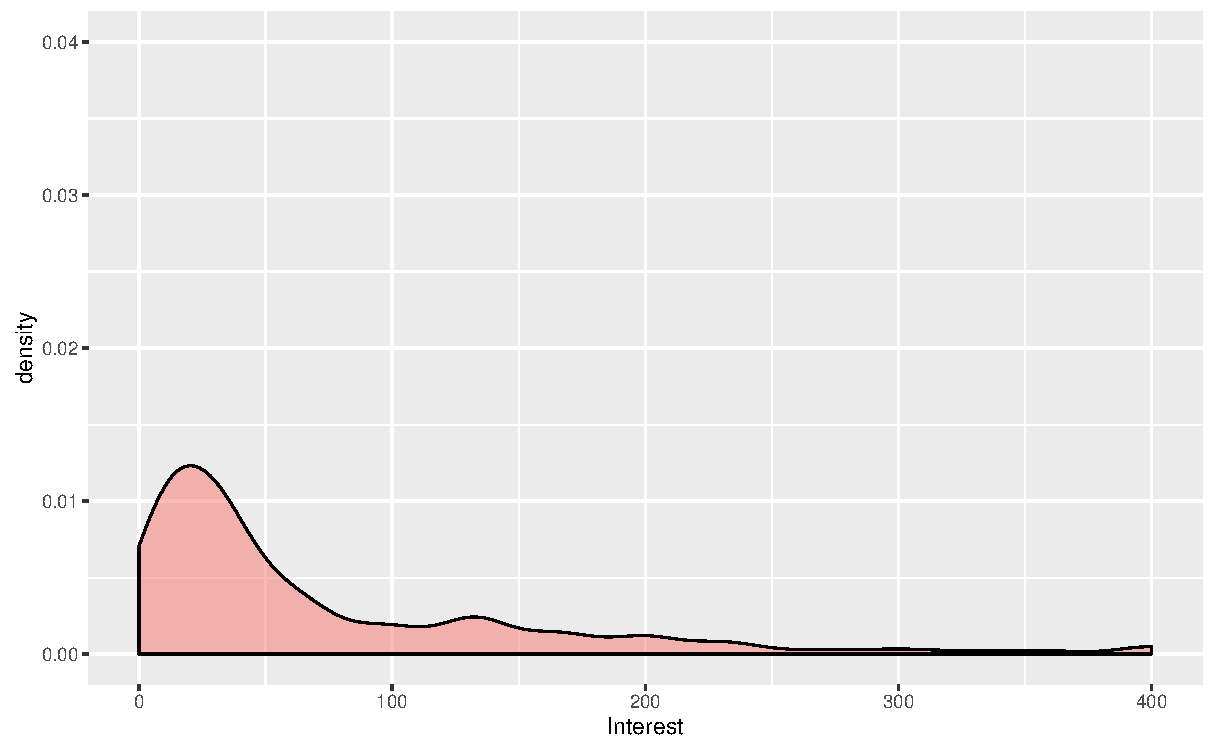
\includegraphics[width=.33\textwidth]{figures/rq1-jruby-non-SATD}
    }
  \end{tabular}
  }
  \scalebox{0.95}{
  \begin{tabular}{ccc}
    \subfigure[Ant (Fan-In)]{ 
      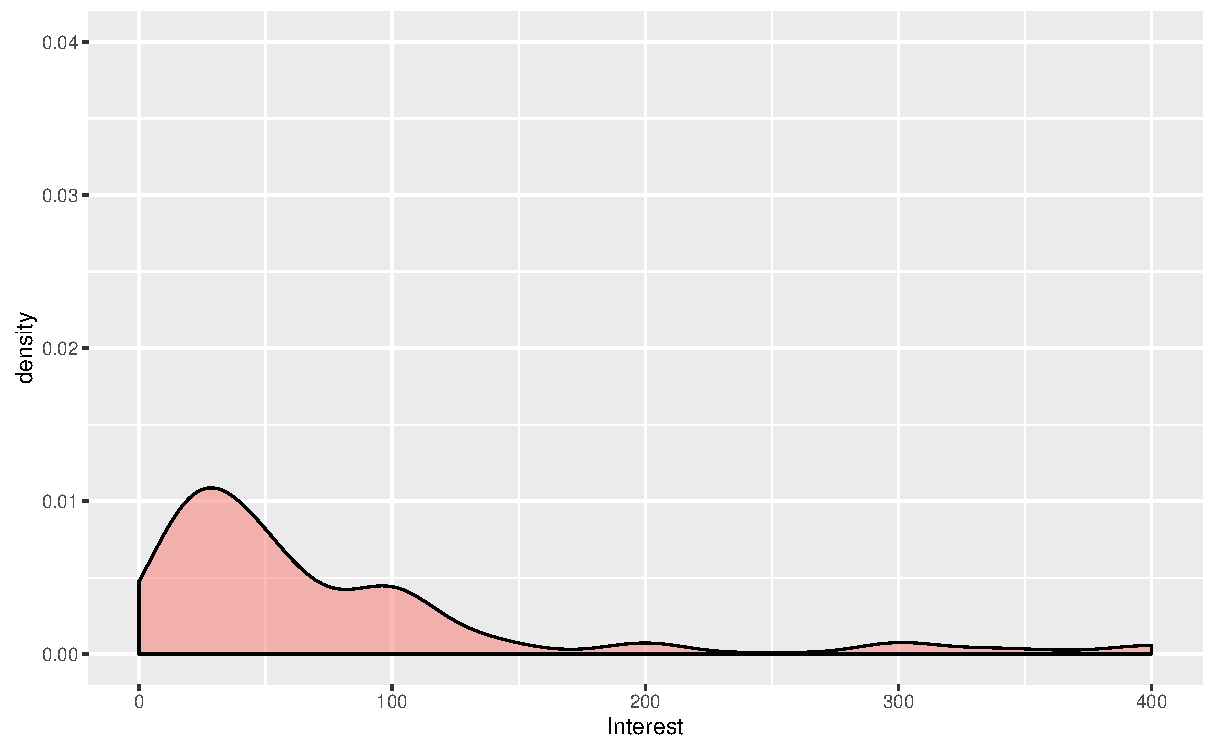
\includegraphics[width=.33\textwidth]{figures/rq1-ant-fanin-non-SATD}
    }
    \subfigure[JMeter (Fan-In)]{ 
      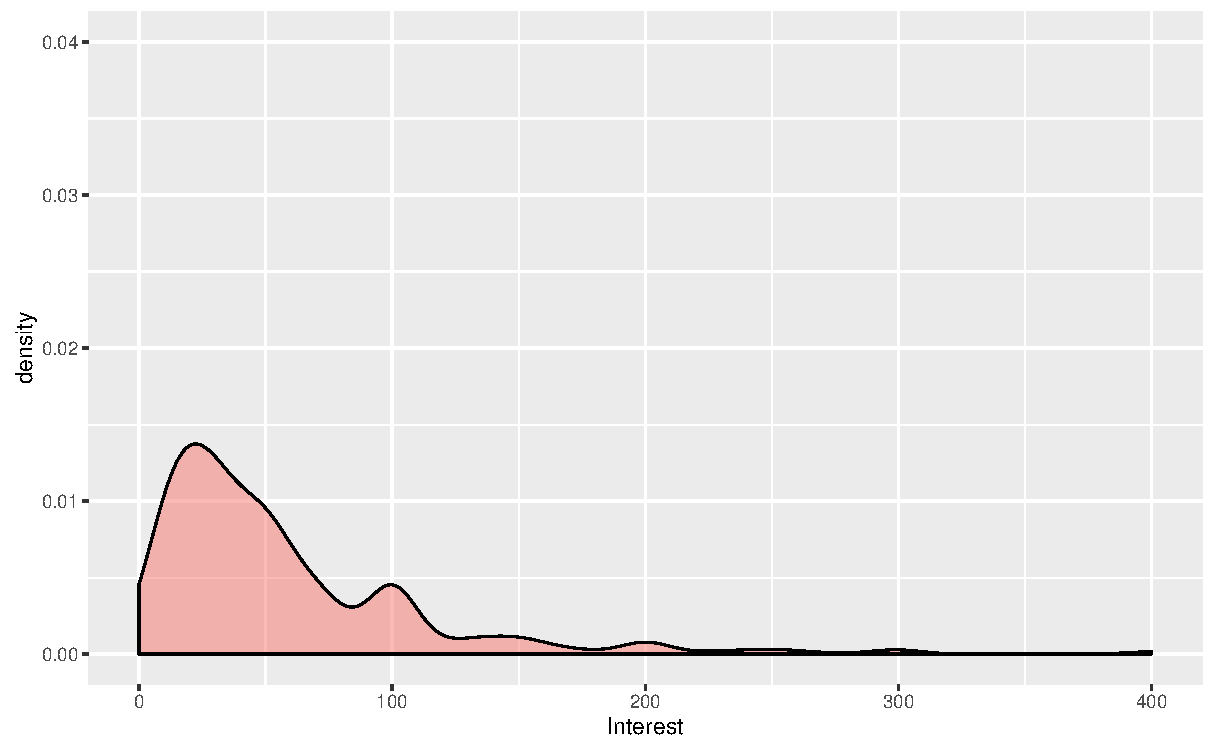
\includegraphics[width=.33\textwidth]{figures/rq1-jmeter-fanin-non-SATD}
    }
    \subfigure[JRuby (Fan-In)]{
      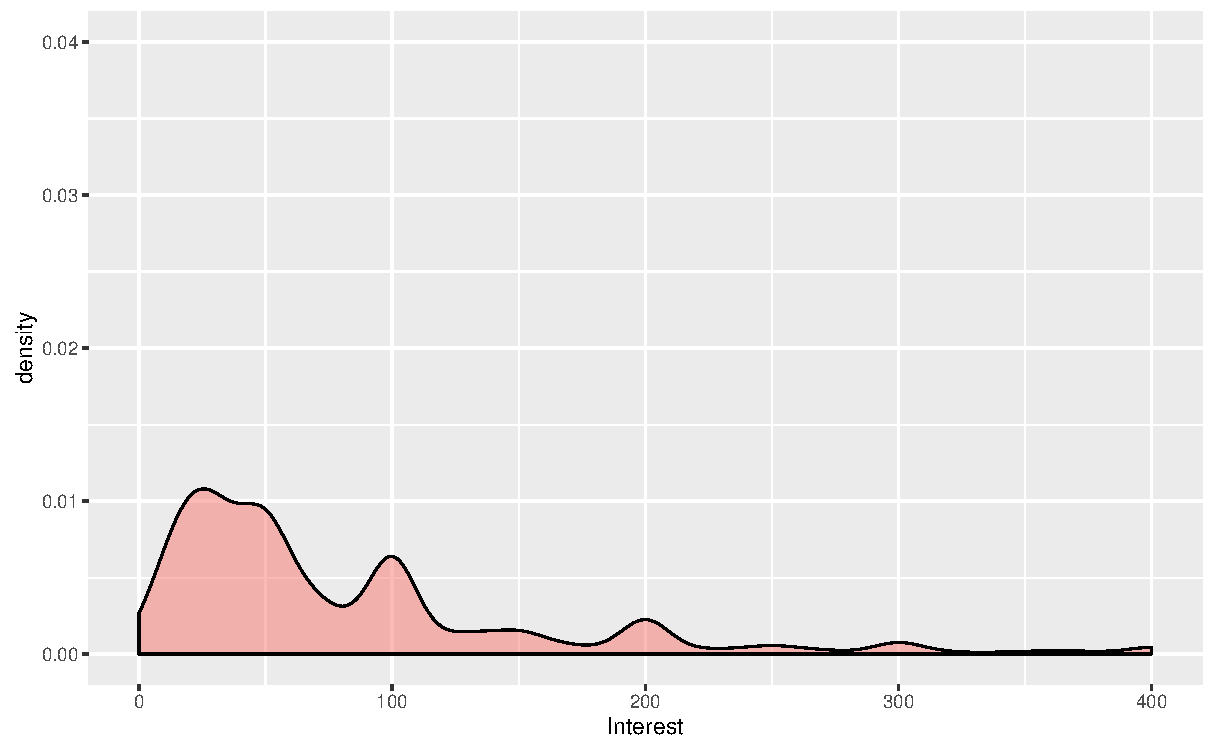
\includegraphics[width=.33\textwidth]{figures/rq1-jruby-fanin-non-SATD}
    }
  \end{tabular}
  }
  \caption{(RQ1) The results of distribution of interest.}
  \label{fig:dist}
  \end{center}
\end{figure*}
%-----------------------------------------------------------------------

\begin{table}[tb]
  \caption{The percentage of SATD that has positive interest for non-SATD}
  \label{tab:percentage_non-SATD}
  \centering

  \begin{tabular}{cl|r|rrr}
  \hline
      &  Project & Positive Rate & All & Positive & Negative \\
  \hline
        & Ant    & 32.3\% & 1,357 &  438  &   196 \\
   LOC  & JMeter & 19.0\% & 4,011 &  763  &   429 \\
        & JRuby  & 16.9\% & 9,983 & 1,686 & 1,827 \\
  \hline
        & Ant    & 22.3\% & 1,245 &   278  &   144 \\
Fan-In  & JMeter & 22.9\% & 3,691 &   845  &   298 \\
        & JRuby  & 32.8\% & 9,390 & 3,084  & 2,079 \\
  \hline
  \end{tabular}
\end{table}

\begin{table}[tb]
  \caption{Statistics}
  \label{tab:statistic_non-SATD}
  \centering

  \begin{tabular}{cl|rrrrr}
  \hline
      &  Project & Min. & 1st Qu. & Median & 3rd Qu. & Max. \\
  \hline
        & Ant    & 1.4 &  12.5 &  28.6  &   83.3 & 1000.0 \\
   LOC  & JMeter & 1.2 &  11.1 &  25.0  &   50.0 & 3060.0 \\
        & JRuby  & 1.1 &  18.2 &  36.4  &  125.0 & 2000.0 \\
  \hline
        & Ant    & 3.0 &  25.0 &  50.3  &  100.0 & 3800.0 \\
Fan-In  & JMeter & 2.4 &  20.0 &  41.3  &   75.0 & 1000.0 \\
        & JRuby  & 0.8 &  33.3 &  60.3  &  133.3 & 8950.0 \\
  \hline
  \end{tabular}
\end{table}

\para{Put the analysis for showing the method that includes more than one technical debt in one version.}